\chapter{Theoretische Grundlagen} \label{chap:theoretical-foundations}

    \section{Additive Fertigung und 3D-Druck}\label{sec:additive-manufacturing-and-3d-printing}
        \subsection{Verfahrensprinzipien der additiven Fertigung}\label{subsec:principles-of-additive-manufacturing}
        Das Grundprinzip der additiven Fertigung ist es, das gewünschte Bauteil durch das gezielte Hinzufügen von Material herzustellen.
        Dies unterscheidet sich grundlegend von subtraktiven Methoden wie der \ac{CNC}-Bearbeitung,
        bei denen Material von einem Rohling abgetragen wird, um die gewünschte Form zu erreichen.
        Es gibt verschiedene Typen der additiven Fertigung.
        \cite{suzukiAdditiveManufacturingVs2024}
        \cite{gibsonAdditiveManufacturingTechnologies2010}
        \cite{yeshiwasReviewArticleAssessment2025}

            \subsubsection{Material Extrusion}
            \ac{FDM} ist ein typisches Material-Extrusionsverfahren.
            Bei diesem Verfahren wird das Material durch eine heiße Düse gedrückt, um es aufzuschmelzen.
            Dieses geschmolzene Material wird Schicht für Schicht aufeinander extrudiert, um so das Bauteil zu erzeugen.
            Durch die schichtweise Zerlegung des Bauteils kann es dazu führen, dass Material frei in der Luft gedruckt werden müsste.
            Um diese Überhänge drucken zu können, werden Stützkonstruktionen benötigt, die nach dem Drucken entfernt werden müssen.
            Beim \ac{FDM}-Drucken wird typischerweise nicht massiv gedruckt, sondern die Füllung zu einem großen Teil hohl gelassen,
            um Zeit und Material zu sparen.
            Für die Form der Füllung sowie der Stützkonstruktion gibt es viele verschiedene Geometrien mit verschiedenen Vor- und Nachteilen.
            Der \ac{FDM}-Druck ist in der Materialwahl hauptsächlich auf Kunststoffe limitiert.
            Es gibt Filamente, bei denen Partikel von anderen Materialien dem Kunststoff beigesetzt werden.
            Eine schematische Darstellung des Verfahrens ist in Abbildung \ref{fig:material-extrusion-process} dargestellt.
            \cite{MaterialExtrusionAdditive}
            \cite{gebhardtAdditiveFertigungsverfahrenAdditive2017}
            \cite{gibsonAdditiveManufacturingTechnologies2010}
            \cite{yeshiwasReviewArticleAssessment2025}
            \sig{Nik Wachsmann}

            \begin{figure}[H]
                \centering
                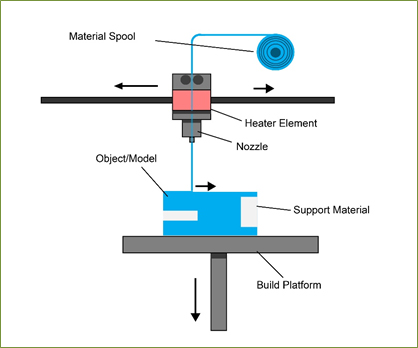
\includegraphics[width=0.4\textwidth]{dependencies/pictures/material extrusion-process.jpg}
                \caption{Schematische Darstellung des Material-Extrusion-Verfahrens (\ac{FDM}). Quelle: \cite{MaterialExtrusionAdditive}}
                \label{fig:material-extrusion-process}
            \end{figure}

            \subsubsection{VAT Photopolymerisation}
            Die VAT Photopolymerisation basiert auf dem gezielten Erhärten von Resin.
            Hierbei wird Schicht für Schicht das Resin aufgetragen und mittels Licht erhärtet, womit es sich mit den darunterliegenden Schichten verbindet.
            Es gibt verschiedene Methoden, wie das genau abläuft.
            Das Bauteil kann nach unten in das Resinbad gelassen werden, wobei das Resin von oben ausgehärtet wird.
            Alternativ steht das Druckbett auf dem Kopf, und das Bauteil wird Schicht für Schicht erzeugt und aus dem Bad gehoben.
            Als Lichtquelle wird entweder ein Laser oder ein Display verwendet.
            Wie bei der Material Extrusion müssen auch hier Stützkonstruktionen verwendet werden.
            Nach dem Drucken müssen die Stützkonstruktionen entfernt werden und das Bauteil muss noch in einer \ac{UV}-Kammer nachgehärtet werden.
            Die grundlegende Prozesskette ist in Abbildung \ref{fig:vat-photopolymerisation-process} dargestellt.
            \cite{VATPhotopolymerisationAdditive}
            \cite{schmidleithnerStereolithography2018}
            \cite{gebhardtAdditiveFertigungsverfahrenAdditive2017}
            \cite{gibsonAdditiveManufacturingTechnologies2010}
            \cite{yeshiwasReviewArticleAssessment2025}
            \sig{Nik Wachsmann}

            \begin{figure}[H]
                \centering
                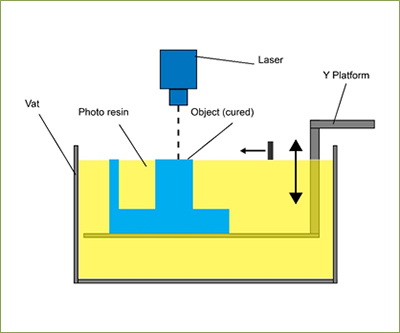
\includegraphics[width=0.4\textwidth]{dependencies/pictures/Photopolymerisation.jpg}
                \caption{Schematische Darstellung der VAT-Photopolymerisation. Quelle: \cite{VATPhotopolymerisationAdditive}}
                \label{fig:vat-photopolymerisation-process}
            \end{figure}

            \subsubsection{Powder Bed Fusion}
            \ac{PBF} ist eine Druckmethode, die nahezu ausschließlich im industriellen Maßstab verwendet wird,
            da diese Maschinen hohe Investitionskosten und einen großen Platzbedarf bedeuten.
            Beim \ac{PBF}-Druck wird Schicht für Schicht ein feines Pulver des Materials aufgetragen und an den
            benötigten Stellen durch Erhitzen verbunden.
            Hierbei gibt es mehrere Methoden, das Material zu erhitzen.
            Entweder wird ein Laser oder ein Elektronenstrahl verwendet.
            Dies bietet einige Vorteile, wie die Möglichkeit, Metalle zu drucken.
            Durch die aufeinanderliegenden Schichten von Pulver werden hierbei keine Stützkonstruktionen benötigt.
            Allerdings haben \ac{PBF}-Drucke typischerweise lange Druckzeiten.
            Aufgrund des Pulvers müssen Bauteile entweder massiv gedruckt werden,
            oder es müssen Löcher in der Wand des Bauteils vorgesehen sein, um das überschüssige Pulver ausschütten zu können.
            Eine schematische Darstellung ist in Abbildung \ref{fig:powder-bed-fusion-process} zu sehen.
            \cite{PowderBedFusion}
            \cite{gebhardtAdditiveFertigungsverfahrenAdditive2017}
            \cite{gibsonAdditiveManufacturingTechnologies2010}
            \cite{yeshiwasReviewArticleAssessment2025}
            \sig{Nik Wachsmann}

            \begin{figure}[H]
                \centering
                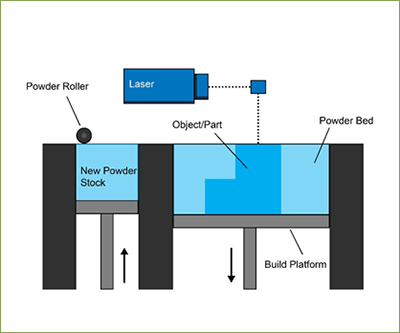
\includegraphics[width=0.4\textwidth]{dependencies/pictures/powderbed_fusion-process.jpg}
                \caption{Schematische Darstellung des Powder-Bed-Fusion-Verfahrens. Quelle: \cite{PowderBedFusion}}
                \label{fig:powder-bed-fusion-process}
            \end{figure}

            \subsubsection{Material Jetting}
            Material Jetting funktioniert ähnlich wie ein herkömmlicher Tintenstrahldrucker,
            jedoch wird anstelle von Tinte ein flüssiges Photopolymer in winzigen Tropfen auf eine Bauplattform aufgetragen.
            Unmittelbar nach dem Auftragen werden die Tropfen durch \ac{UV}-Licht ausgehärtet.
            Da der Druckkopf über hunderte Düsen verfügt, können unterschiedliche Materialien oder Farben gleichzeitig verarbeitet werden,
            was den Druck von Bauteilen mit verschiedenen Härten oder Transparenzen ermöglicht.
            Die Oberflächenqualität ist hierbei sehr hoch.
            Ähnlich wie bei der Photopolymerisation müssen Stützstrukturen verwendet werden, die jedoch oft aus einem speziellen,
            leicht löslichen Material bestehen.
            Der prinzipielle Ablauf ist in Abbildung \ref{fig:material-jetting-process} dargestellt.
            \cite{MaterialJettingAdditive}
            \cite{gebhardtAdditiveFertigungsverfahrenAdditive2017}
            \cite{WhatMaterialJetting}
            \sig{Nik Wachsmann}
            
            \begin{figure}[H]
                \centering
                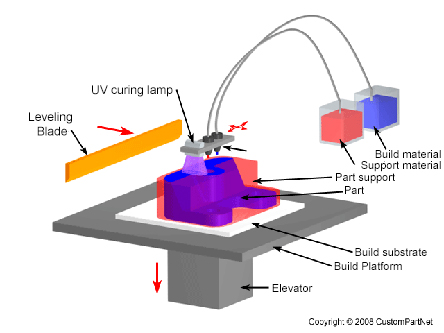
\includegraphics[width=0.4\textwidth]{dependencies/pictures/material_jetting_process.jpg}
                \caption{Schematische Darstellung des Material-Jetting-Verfahrens. Quelle: \cite{MaterialJettingAdditive}}
                \label{fig:material-jetting-process}
            \end{figure}


            \subsubsection{Binder Jetting}
            Beim Binder Jetting werden pulverförmiger Werkstoff und ein flüssiges Bindemittel kombiniert.
            Eine Walze verteilt zunächst eine dünne Pulverschicht auf dem Druckbett.
            Anschließend trägt ein Druckkopf das Bindemittel gezielt dort auf, wo das Bauteil entstehen soll,
            um die Pulverkörner zu verkleben.
            Da das Bauteil während des Prozesses vom umliegenden Pulver gestützt wird,
            sind keine zusätzlichen Stützkonstruktionen erforderlich.
            Nach dem Druck befindet sich das Bauteil im sogenannten „Grünzustand“ und ist noch sehr fragil.
            Es muss daher in einem anschließenden Prozessschritt in einem Ofen gesintert oder mit einem anderen Material infiltriert werden,
            um seine endgültige Festigkeit zu erreichen.
            Eine schematische Darstellung des Verfahrens ist in Abbildung \ref{fig:binder-jetting-process} enthalten.
            \cite{BinderJettingAdditive}
            \cite{gebhardtAdditiveFertigungsverfahrenAdditive2017}
            \sig{Nik Wachsmann}

            \begin{figure}[H]
                \centering
                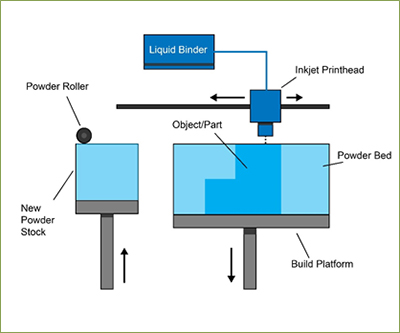
\includegraphics[width=0.4\textwidth]{dependencies/pictures/binderjetting-process.jpg}
                \caption{Schematische Darstellung des Binder-Jetting-Verfahrens. Quelle: \cite{BinderJettingAdditive}}
                \label{fig:binder-jetting-process}
            \end{figure}

            \subsubsection{Sheet Lamination}
            Die Sheet Lamination umfasst Verfahren, bei denen dünne Materialschichten wie meist Metallfolien,
            Papier oder Kunststoffplatten übereinandergelegt und miteinander verbunden werden.
            Die Verbindung erfolgt je nach Material durch Klebstoff, thermisches Verschweißen oder mittels Ultraschall.
            Nach dem Verbinden der Schichten wird die gewünschte Kontur jeder Lage mit einem Laser oder einem Fräswerkzeug ausgeschnitten.
            Da das Bauteil aus fertigen Schüttgut-Platten oder Folien entsteht, ist die Materialvielfalt groß.
            Allerdings ist der Materialabfall im Vergleich zu anderen Verfahren höher,
            da das nicht benötigte Material der Platten nach dem Prozess entfernt werden muss.
            Das schematische Prinzip ist in Abbildung \ref{fig:sheet-lamination-process} dargestellt.
            \cite{SheetLaminationAdditive}
            \cite{gebhardtAdditiveFertigungsverfahrenAdditive2017}
            \cite{gibsonAdditiveManufacturingTechnologies2010}
            \sig{Nik Wachsmann}

            \begin{figure}[H]
                \centering
                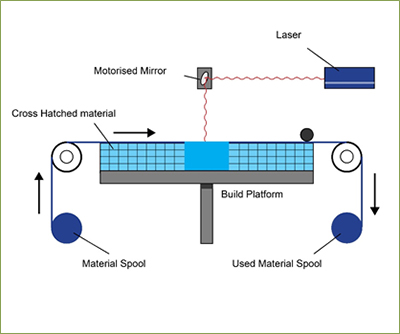
\includegraphics[width=0.4\textwidth]{dependencies/pictures/sheet_lamination-process.jpg}
                \caption{Schematische Darstellung des Sheet-Lamination-Verfahrens. Quelle: \cite{SheetLaminationAdditive}}
                \label{fig:sheet-lamination-process}
            \end{figure}
        
        \subsection{Nachteile der planaren Bahnplanung}\label{subsec:disadvantages-of-planar-slicing}
        Alle in Abschnitt \ref{sec:additive-manufacturing-and-3d-printing} beschriebenen Fertigungsverfahren beruhen auf dem schichtweisen Aufbauen des Bauteils.
        Dies führt zu sehr guter Materialverbindung innerhalb der Schichten, jedoch ist der Verbund zwischen den Schichten eine Schwachstelle.
        Die Planarität und Parallelität der Schichten führen dadurch zu Schwäche in eine Richtung.
        Bei Schichten, die in der X-Z Achse liegen und in Y Achse aufeinander gesetzt werden, ist die Zugfestigkeit in Y-Achse geringer als in X- und Z-Achsen.
        Dieses Phänomen wird Anisotropie genannt und ist bei allen zuvor genannten Verfahren zu beobachten.
        Zusätzlich werden bei den Verfahren, bei denen das Material nicht selbststützend ist, zusätzlich Stützkonstruktionen benötigt.
        Diese verwendet mehr Material, kann zu höheren Druckzeiten führen, und erhöht die benötigte Nachbearbeitung.
        \cite{megersaInvestigationInfluenceFused2024}
        \cite{asimOptimization3DPrinting2025}
        \cite{toprakOptimizationTensileStrength2024}
        \cite{chabanIsotropicVsAnisotropic2025}
        \cite{huNonplanarAdditiveManufacturing2026}
        \sig{Nik Wachsmann}

        \subsection{Geometrische Überhangdefinition}\label{subsec:overhang-definition}
        Als \emph{Überhang}\index{Überhang!Definition} wird ein Bauteilbereich bezeichnet,
        der bei planarer Fertigung ohne Unterstützung durch Material einer darunterliegenden Schicht
        in freier Luft extrudiert werden müsste.
        Die geometrische Grundlage für die Überhangdetektion bildet der Winkel zwischen der
        nach außen zeigenden Einheitsnormalen $\hat{n}$ einer Dreiecksfläche und dem Einheitsvektor
        der Baurichtung $\hat{a}$ (üblicherweise $+\vec{e}_z$).
        Der Winkel $\phi$ zwischen $\hat{n}$ und $\hat{a}$ ergibt sich zu:
        \begin{equation}
            \phi \;=\; \arccos\!\bigl(\hat{n} \cdot \hat{a}\bigr)
            \label{eq:overhang-angle}
        \end{equation}
        Für $\phi < 90\degree$ zeigt die Normale in Richtung der Bauachse; die Fläche ist nach oben geneigt und selbststützend.
        Für $\phi > 90\degree$ zeigt die Normale von der Bauachse weg; die Fläche ist nach unten geneigt
        und bildet einen potenziellen Überhang.
        Aus experimentellen Untersuchungen mit typischen \ac{FDM}-Werkstoffen ergibt sich ein kritischer
        Grenzwinkel $\alpha$ (typischerweise $\alpha \approx 45\degree$ zur Horizontalen),
        bis zu dem das Material aufgrund seiner Viskosität selbsttragend ist.
        Formal liegt ein stützpflichtiger Überhang vor, wenn:
        \begin{equation}
            \phi \;>\; 90\degree + \alpha
            \label{eq:critical-overhang}
        \end{equation}
        wobei $\alpha$ den parametrierbaren Grenzwinkel bezeichnet.
        Beim 6-achsigen Druck lässt sich durch gezielte Neuausrichtung der Werkzeugachse $\hat{a}$
        erreichen, dass $\phi$ lokal unterhalb des kritischen Grenzwinkels bleibt,
        sodass Stützkonstruktionen entfallen.
        \cite{gorskiExperimentalDeterminationCritical2015}
        \cite{vanekCleverSupportEfficient2014}
        \sig{Nik Wachsmann}

        \subsection{Multiaxis und Nichtplanares Slicing}\label{subsec:planar-and-non-planar-slicing}
        Es gibt einen Unterschied zwischen dem Multiaxis und dem nichtplanaren Slicing.
        Der Multiachs Druck besteht aus vielen planaren Schichten, die jedoch nicht alle parallel zueinander liegen.
        Da die einzelnen Schichten immer noch planar sind, ist dies kein nichtplanares Slicing.
        Der Base Algorithmus ist ein Beispiel hierfür.
        Beim nichtplanaren Slicen sind die einzelnen Schichten nicht Planar.
        Hierfür sind sowohl der Kugel- als auch der Kristall Algorithmus Beispiele.
        Der Unterschied ist in \cref{fig:multiaxis-vs-nonplanar} zu sehen.
        \cite{nayyeriPlanarNonplanarSlicing2022}
        \cite{huNonplanarAdditiveManufacturing2026}
        \begin{figure}[H]
            \centering
            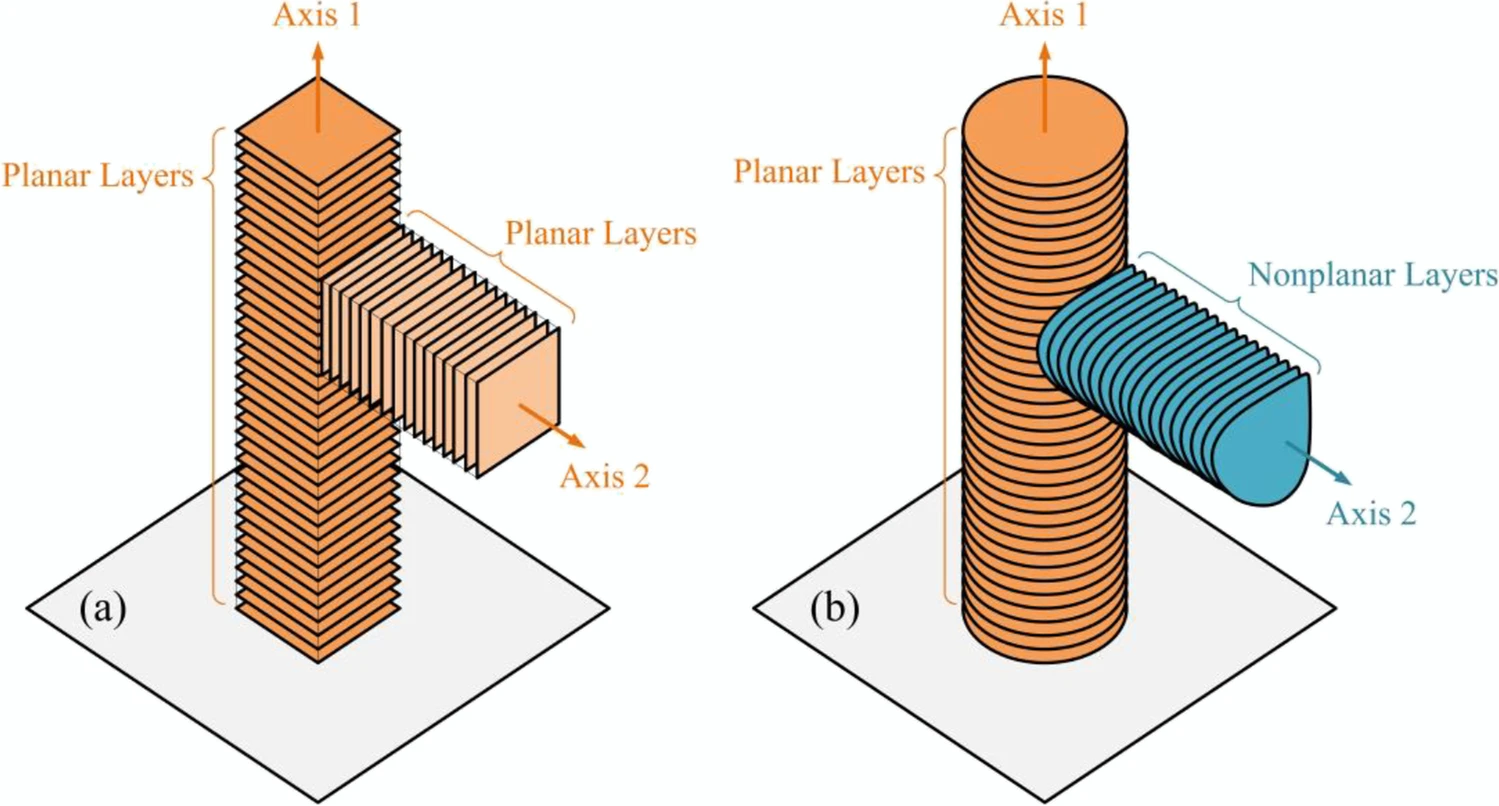
\includegraphics[width=0.5\textwidth]{dependencies/pictures/multiaxis_vs_nonplanar.png}
            \caption{Unterschied zwischen Multiachs und Nichtplanarem Slicing. Quelle: \cite{nayyeriPlanarNonplanarSlicing2022c}}
            \label{fig:multiaxis-vs-nonplanar}
        \end{figure}
        \sig{Nik Wachsmann}


        \subsection{Additive Fertigung für den 6-Achsigen Druck}
        Aus den erwähnten additiven Fertigungsmethoden ist für den 6-achsigen Druck nur die Material Extrusion sinnvoll.
        Bei diesem Verfahren ist es möglich, von verschiedenen Seiten an das Bauteil zu extrudieren.
        Bei \ac{PBF} ist es nur möglich, von oben auf das Bauteil zu extrudieren.
        Die beiden Jetting-Methoden sind von der Schwerkraft abhängig, um das Material zu verteilen.
        Sheet Lamination ist nur mit planaren Schichten realistisch.
        Es wäre möglich, bei der VAT Photopolymerisation das von oben kommende Druckbett zu rotieren.
        Jedoch sind auch dann nur planare Schichten möglich, was den erhöhten Aufwand nicht wert ist.
        Aus diesen Gründen wird für dieses Projekt die Material Extrusion verwendet.
        \cite{gibsonAdditiveManufacturingTechnologies2010}
        \cite{huNonplanarAdditiveManufacturing2026}
        \sig{Nik Wachsmann}

        \subsection{Seitlicher Materialauftrag bei der Materialextrusion}\label{subsec:sideways-material-extrusion}
        Ein wesentlicher Vorteil der Material Extrusion für den 6-achsigen Druck ist,
        dass das abgelegte Material nicht wie eine frei fließende Flüssigkeit reagiert.
        Das aufgeschmolzene Thermoplast wird zwar in viskosem Zustand extrudiert,
        haftet nach dem Austritt aus der Düse jedoch unmittelbar an der zuvor gedruckten Bahn oder an der Bauteiloberfläche.
        Gleichzeitig kühlt das Material schnell ab und verfestigt sich innerhalb kurzer Zeit,
        sodass es seine Form weitgehend beibehält.
        Dadurch kann auch von der Seite auf das Bauteil gedruckt werden,
        ohne dass das Material direkt von der Oberfläche wegtropft.
        Diese Eigenschaft ist eine zentrale Voraussetzung dafür,
        die Freiheitsgrade eines 6-Achs-Systems für nichtplanare und mehrachsige Bahnstrategien auszunutzen.
        Dennoch bleibt die Schwerkraft ein relevanter Einflussfaktor,
        weshalb die mögliche Werkzeugorientierung weiterhin von Prozessparametern wie Temperatur,
        Extrusionsrate, Bahngeschwindigkeit und dem Abstand zur Oberfläche abhängt.
        \sig{Nik Wachsmann}


        \subsection{Prozesskette im materialextrusionsbasierten 3D-Druck}\label{subsec:process-chain-in-material-extrusion-3d-printing}
        Zu Beginn des Prozesses steht die Erstellung eines digitalen 3D-Modells.
        Wie bei der subtraktiven Fertigung müssen auch hier fertigungsrelevante Toleranzen berücksichtigt werden.
        Das fertige Modell wird anschließend in einem Slicing-Programm verarbeitet und in \ac{GCODE} umgewandelt.
        Dieser \ac{GCODE} ist maschinenspezifisch, da bereits beim Slicen die Parameter des Ziel-Druckers festgelegt werden müssen.
        Im letzten Schritt führt der Drucker diesen Code aus und baut das Bauteil Schicht für Schicht auf.
        \cite{gibsonAdditiveManufacturingTechnologies2010}
        \cite{yeshiwasReviewArticleAssessment2025}
        \sig{Nik Wachsmann}

        \subsection{Qualitätsrelevante Prozessgrößen}\label{subsec:quality-relevant-process-variables}
        Die Qualität des Bauteils wird durch verschiedene Prozessgrößen maßgeblich beeinflusst.
        Die entscheidenden Parameter sind die Schichtdicke und der Düsendurchmesser (Nozzle-Durchmesser).
        Eine größere Schichtdicke reduziert die Herstellungszeit, führt jedoch zu einer geringeren Auflösung und einer stärkeren Stufenbildung an vertikalen Rundungen.
        Statt einer konstanten Schichtdicke kann auch eine adaptive Schichthöhe verwendet werden.
        Dabei wird die Layerhöhe in Abhängigkeit von der lokalen Bauteilgeometrie variiert,
        um in stark gekrümmten oder detailreichen Bereichen eine höhere Auflösung zu erreichen
        und in geometrisch einfachen Bereichen die Fertigungszeit zu reduzieren.
        Gerade beim nichtplanaren Slicing ist dies relevant,
        da sich die lokale Schichtgeometrie entlang des Pfades ändern kann und eine konstante Layerhöhe
        die erreichbare Oberflächenqualität oder Prozessstabilität unnötig einschränken würde.
        Ein größerer Düsendurchmesser beschleunigt den Druckprozess ebenfalls, resultiert jedoch in einer gröberen Auflösung der Slices und stärker abgerundeten Ecken.
        Weitere Stellgrößen sind die Druckgeschwindigkeit und die Temperatur des Druckkopfes.
        Zudem wirken sich externe Faktoren wie die mechanische Präzision des Druckers sowie Umgebungsbedingungen (Lufttemperatur und Feuchtigkeit) auf das Ergebnis aus.
        \cite{gibsonAdditiveManufacturingTechnologies2010}
        \cite{ahmadSystematicReviewFused2022}
        \sig{Nik Wachsmann}

    \section{Slicing und Bahnplanung}\label{sec:slicing-and-path-planning}
        \subsection{Polygonale Geometrierepräsentation}\label{subsec:polygonal-geometry-representation}
        Alle in dieser Arbeit betrachteten Slicing-Algorithmen operieren auf dreidimensionalen Dreiecksnetzen.
        Ein Dreiecksnetz $\mathcal{M} = (V, F)$ besteht aus einer Menge von Vertizes
        $V = \{\vec{v}_1, \dots, \vec{v}_{|V|}\} \subset \mathbb{R}^3$
        und einer Menge von Dreiecken $F \subseteq \binom{[|V|]}{3}$,
        wobei jedes Dreieck durch drei ganzzahlige Vertex-Indizes beschrieben wird.
        In der \textbf{indizierten Dreiecksrepräsentation} werden Vertexpositionen einmalig gespeichert
        und Dreiecke ausschließlich über Indizes referenziert,
        sodass gemeinsam genutzte Vertizes nicht dupliziert werden.

        \textbf{Adjazenzstrukturen.}
        Für Slicing und Normalenberechnung werden Nachbarschaftsbeziehungen benötigt.
        Die Vertex-zu-Flächen-Adjazenz $\mathcal{F}(i)$ listet alle Dreiecke, die an Vertex $i$ anliegen;
        aus ihr lassen sich in $\mathcal{O}(|F|)$ auch die Kanten-zu-Flächen-Beziehungen ableiten.

        \textbf{Vertex Normalen.}
        Die Normalen einzelner Dreiecke sind an gemeinsamen Kanten unstetig.
        Für eine glatte Approximation werden flächengewichtete Vertex Normalen gebildet:
        \begin{equation}
            \hat{n}_i
            \;=\;
            \frac{\displaystyle\sum_{f \in \mathcal{F}(i)} A_f \,\hat{n}_f}
                 {\displaystyle\left\|\sum_{f \in \mathcal{F}(i)} A_f \,\hat{n}_f\right\|}
            \label{eq:vertex-normal}
        \end{equation}
        wobei $A_f$ der Flächeninhalt und $\hat{n}_f$ die Einheitsnormale des anliegenden Dreiecks $f$ ist.
        Diese Vertex-Normalen werden im Slicing entlang der Schnittkanten interpoliert,
        um Werkzeugorientierungen an jedem Bahnpunkt abzuleiten.

        \textbf{Mannigfaltigkeit und Wasserdichtheit.}
        Ein Netz gilt als \emph{mannigfaltig} (engl.\ \emph{manifold}),
        wenn jede Kante von genau zwei Dreiecken geteilt wird
        und die an jedem Vertex anliegenden Dreiecke einen einfach zusammenhängenden Fächer bilden.
        Ein mannigfaltiges, lückenlos geschlossenes Netz heißt \emph{wasserdicht}.
        Diese Eigenschaft ist für alle Slicing-Verfahren dieser Arbeit erforderlich,
        da nicht mannigfaltige Netze bei Schnitten offene oder mehrdeutige Konturen erzeugen.

        \textbf{\ac{STL}-Format.}
        Das in der additiven Fertigung weitverbreitete Eingangsformat ist \ac{STL}.
        Eine \ac{STL}-Datei enthält für jedes Dreieck drei Eckpunkte und eine Flächennormale,
        jedoch keinerlei Topologie- oder Adjazenzinformationen -- man spricht von einer \emph{Triangle Soup}.
        Da benachbarte Dreiecke gemeinsame Vertices als separate Einträge abspeichern,
        ist nach dem Import ein \emph{Vertex-Welding}-Schritt notwendig:
        positionsgleiche Vertizes werden zusammengeführt, um die indizierten Adjazenzstrukturen aufzubauen.
        \cite{lettoriReviewGeometryRepresentation2022}
        \cite{gregoriSlicingTriangleMeshes2014}
        \sig{Nik Wachsmann}

        \subsection{Slicing-Strategien und Schichtmodellierung}\label{subsec:slicing-strategies-and-layer-modeling}
        Für den planaren 3D-Druck wird das Netz des zu druckenden Objekts zunächst in planare 2D-Schichten geteilt.
        Nach dieser Transformation wird für jede dieser Schichten berechnet, wie das Material verteilt wird.
        In klassischen Slicern ist die Schichtdicke dabei häufig global konstant,
        während fortgeschrittene Verfahren variable oder adaptive Schichthöhen einsetzen,
        um die Diskretisierung an die lokale Geometrie des Bauteils anzupassen.
        Bei nichtplanaren Slicing-Strategien kann diese Anpassung zusätzlich entlang gekrümmter Pfade erfolgen,
        sodass sich nicht nur die Orientierung der Schichten, sondern auch deren lokale Höhe verändert.
        Hierbei werden die Slices nicht vollständig ausgefüllt.
        Um Material und Druckzeit zu sparen, werden 3D-gedruckte Bauteile, zumindest beim \ac{FDM}-Druck, nicht massiv gedruckt.
        Um die Stabilität des Bauteils dennoch zu gewährleisten, werden die Wände massiv gedruckt.
        Hierbei werden die ersten und letzten Schichten massiv gedruckt.
        Die Anzahl dieser massiven Schichten hängt von der Wanddicke ab.
        Diese bilden die oberen und unteren Wände.
        Für die anderen Wände werden mehrere Materiallinien um den Umfang des Slices gelegt.
        Im Inneren wird viel Volumen frei gelassen.
        Für die Füllung gibt es viele verschiedene Geometrien mit unterschiedlichen Vor- und Nachteilen.
        \cite{palinkasTYPESAPPLICATIONINFILL}
        \cite{sapkotaReviewFusedDeposition2024}
        \sig{Nik Wachsmann}

        \subsection{Bahnplanung für Extrusionsprozesse}\label{subsec:path-planning-for-extrusion-processes}
        Nachdem alle Schichten berechnet sind, werden die Toolpaths berechnet.
        Diese sagen aus, wie sich der Druckkopf des Druckers bewegen soll.
        In dem Zusammenhang wird auch die Extrusion mitberechnet.
        Abhängig von der Geschwindigkeit des Druckkopfs und der Höhe der Schichten muss mehr oder weniger Material extrudiert werden.
        Wenn sich der Druckkopf zu einem neuen Punkt bewegen muss, ohne dabei zu drucken, muss der Materialfluss gestoppt werden.
        Aus diesem Grund ist es nicht möglich, einfach einen konstant drehenden Motor für den Materialvorschub zu verwenden.
        Bei der Bahnplanung muss auch die Beschleunigung des Druckkopfes beachtet werden.
        Bei zu hoher Druckgeschwindigkeit oder zu scharfen Kanten kann es durch die schnelle Geschwindigkeitsänderung des Kopfes zu Vibrationen im Drucker kommen.
        Diese sollten bei der Bahnplanung möglichst reduziert oder zumindest berücksichtigt werden.
        Manche Hochgeschwindigkeitsdrucker erfassen diese Vibrationen und gleichen sie während des Druckens aus.
        \cite{ResonanceCompensationKlipper}
        \sig{Nik Wachsmann}
        
        \subsection{Maschinennahe Befehlsformate und \texorpdfstring{\ac{GCODE}}{G-Code}}\label{subsec:machine-near-command-formats-and-gcode}
        Um den 3D-Drucker anzusteuern, muss die Abstraktion der Bahnplanung auf das Druckermodell abgebildet werden.
        Um dies zu erreichen, wird typischerweise das \ac{GCODE}-Format verwendet.
        Das \ac{GCODE}-Format besteht aus einer sequentiellen Liste von Befehlen, die der Maschinensteuerung Anweisungen über Positionierung, Geschwindigkeiten und Hilfsfunktionen geben.
        Diese Befehle enthalten mehrere Informationen, die für das korrekte Abfahren der geplanten Bahn benötigt werden.
        Dazu gehören unter anderem die Art des Befehls, die Zielposition sowie die Extrusions- und Bewegungsgeschwindigkeit.
        \sig{Nik Wachsmann}

        \subsection{Diskrete Differentialgeometrie und harmonische Skalarfelder}\label{subsec:harmonic-scalar-fields}
        Eine der zentralen Datenstrukturen des in \cref{subsec:concept-crystal-algorithm} beschriebenen
        Kristall-Algorithmus ist ein harmonisches Skalarfeld $\Phi$, das auf dem Dreiecksnetz
        des Bauteils gelöst wird.
        Die theoretische Grundlage bildet der \textbf{Laplace-Beltrami-Operator},
        das natürliche Analogon des klassischen Laplace-Operators auf gekrümmten Flächen.

        \textbf{Harmonische Funktionen.}
        Eine skalare Funktion $\Phi \colon V \to \mathbb{R}$ heißt \emph{harmonisch},
        wenn sie die Laplace-Gleichung erfüllt:
        \begin{equation}
            \Delta \Phi \;=\; 0
            \label{eq:laplace}
        \end{equation}
        Harmonische Funktionen besitzen das \emph{Maximumprinzip}:
        ihre Extrema liegen ausschließlich auf dem Rand des Definitionsbereichs.
        Dadurch verläuft $\Phi$ monoton zwischen den vorgegebenen Dirichlet-Randbedingungen,
        was eine lückenlose, stufenlose Überdeckung des Bauteils garantiert.
        Die Niveauflächen $\Phi = \mathrm{const}$ liefern glatte, ineinander übergehende Schichten
        als natürliche Slicing-Ebenen.

        \textbf{Diskretisierung durch Kotangensgewichte.}
        Auf einem gegebenen Dreiecksgitter wird $\Delta\Phi = 0$ durch das lineare Gleichungssystem
        \begin{equation}
            \bigl(L\,\boldsymbol{\phi}\bigr)_i \;=\; 0, \qquad i \in V_{\mathrm{frei}}
            \label{eq:discrete-laplace}
        \end{equation}
        ersetzt, wobei $\boldsymbol{\phi} \in \mathbb{R}^{|V|}$ den Vektor der Knotenwerte bezeichnet.
        Die \textbf{Kotangenten-Laplace-Matrix} $L$ ist definiert durch:
        \begin{equation}
            L_{ij} \;=\;
            \begin{cases}
                \tfrac{1}{2}\!\left(\cot\alpha_{ij} + \cot\beta_{ij}\right) & \text{falls } (i,j) \in E \\
                -\displaystyle\sum_{k \sim i} L_{ik} & \text{falls } i = j \\
                0 & \text{sonst}
            \end{cases}
            \label{eq:cotangent-laplacian}
        \end{equation}
        Dabei sind $\alpha_{ij}$ und $\beta_{ij}$ die Winkel, die der Kante $(i,j)$
        in den beiden anliegenden Dreiecken gegenüberliegen.
        Die Matrix $L$ ist symmetrisch, positiv semidefinit und dünnbesetzt ($\mathcal{O}(|V|)$ Nicht-Null-Einträge),
        was eine effiziente Lösung über direkte Sparse-Solver ermöglicht.
        Für quasi-uniforme Vernetzungen konvergiert $L$ gegen den kontinuierlichen Laplace-Beltrami-Operator.
        \cite{wardetzkyDiscreteLaplaceOperators2007}
        \sig{Nik Wachsmann}

    \section{Robotikgrundlagen für den 6-Achs-3D-Druck}\label{sec:robotics-foundations-for-6-axis-3d-printing}
        \subsection{Kinematische Modellierung serieller Roboter}\label{subsec:kinematic-modeling-of-serial-robots}
        Im Gegensatz zu klassischen Drei-Achs-Druckern, die meist auf kartesischen Portalsystemen basieren, nutzen serielle Roboter eine Kette von Rotationsachsen.
        Dieses Verfahren wird Vorwärtskinematik genannt.
        Hierbei wird für jedes Glied ein lokales Koordinatensystem definiert,
        um die Transformation von der Roboterbasis bis zum Werkzeugmittelpunkt über eine Multiplikation von Transformationsmatrizen zu berechnen.
        Mit Vorwärtskinematik ist es kompliziert, flüssige Bewegungen zu erzeugen, welche für den 3D-Druck wichtig sind.

        Die mathematische Grundlage hierfür bildet die \textbf{\ac{DH}\- Konvention}.
        Jedem Gelenk $i$ werden vier Parameter zugeordnet:
        die Gliedlänge $a_i$, die Gliedtorsion $\alpha_i$, den Gelenkoffset $d_i$ sowie den Gelenkwinkel $\theta_i$,
        der bei Drehgelenken die variable Größe ist.
        Aus diesen vier Parametern ergibt sich die homogene $4 \times 4$-Transformationsmatrix zwischen zwei aufeinanderfolgenden Koordinatensystemen:
        \begin{equation}
            ^{i-1}T_i =
            \begin{pmatrix}
                \cos\theta_i & -\sin\theta_i\cos\alpha_i &  \sin\theta_i\sin\alpha_i & a_i\cos\theta_i \\
                \sin\theta_i &  \cos\theta_i\cos\alpha_i & -\cos\theta_i\sin\alpha_i & a_i\sin\theta_i \\
                0            &  \sin\alpha_i             &  \cos\alpha_i             & d_i             \\
                0            &  0                        &  0                        & 1
            \end{pmatrix}
            \label{eq:dh-matrix}
        \end{equation}
        Die Gesamttransformation vom Basiskoordinatensystem zum Werkzeugmittelpunkt (\ac{TCP}) ergibt sich
        durch Multiplikation aller $n$ Einzelmatrizen:
        \begin{equation}
            ^0T_n = \prod_{i=1}^{n} {}^{i-1}T_i = {}^0T_1 \cdot {}^1T_2 \cdots {}^{n-1}T_n
            \label{eq:forward-kinematics}
        \end{equation}
        Das Ergebnis $^0T_n \in \mathbb{R}^{4 \times 4}$ enthält in seiner linken oberen $3 \times 3$-Teilmatrix die Rotationsmatrix $R$
        und in der vierten Spalte den Positionsvektor $\mathbf{p}$ des \ac{TCP} im Basiskoordinatensystem.
        \cite{craigIntroductionRoboticsMechanics2005}
        \sig{Nik Wachsmann}

        \subsection{Inverse Kinematik und Singularitäten}\label{subsec:inverse-kinematics-and-singularities}
        Um die Steuerung eines Roboters in einem kartesischen Koordinatensystem durchführen zu können, wird inverse Kinematik benötigt.
        Bei der inversen Kinematik werden für einen gegebenen Punkt im dreidimensionalen Raum die Gelenkwinkel berechnet, um den Werkzeugmittelpunkt an diesen Punkt zu bringen.
        Hierbei gibt es in den meisten Fällen mehrere Positionen, die der Roboterarm einnehmen kann, der die gewünschte Zielposition erreicht.
        Der Algorithmus muss aus diesen Optionen diejenige auswählen, die in der aktuellen Situation am logischsten ist.
        Hierbei muss beachtet werden, wie der Roboter sich in die Position bewegt und wie er sich danach weiter bewegen kann.

        \textbf{Jacobi-Matrix und numerische Lösung.}
        Die Beziehung zwischen Gelenk- und kartesischen Geschwindigkeiten wird durch die \textbf{Jacobi-Matrix}
        $J(\mathbf{q}) \in \mathbb{R}^{6 \times n}$ beschrieben:
        \begin{equation}
            \dot{\mathbf{x}} = J(\mathbf{q})\,\dot{\mathbf{q}}
            \label{eq:jacobian}
        \end{equation}
        Hierbei ist $\dot{\mathbf{x}} \in \mathbb{R}^6$ der Vektor der kartesischen Geschwindigkeiten (Translation und Rotation des \ac{TCP})
        und $\dot{\mathbf{q}} \in \mathbb{R}^n$ der Gelenkgeschwindigkeitsvektor.
        Für einen gegebenen Positionsfehler $\Delta\mathbf{x}$ ergibt sich die notwendige Gelenkwinkeländerung iterativ über
        die Moore-Penrose-Pseudoinverse $J^+$:
        \begin{equation}
            \Delta\mathbf{q} = J^+(\mathbf{q})\,\Delta\mathbf{x},
            \qquad J^+ = J^T\bigl(J J^T\bigr)^{-1}
            \label{eq:pseudoinverse}
        \end{equation}
        Diese Iteration wird so lange wiederholt, bis $\|\Delta\mathbf{x}\|$ unterhalb einer definierten Toleranz liegt.
        Analytische Lösungen existieren für bestimmte Robotergeometrien (z.\,B. Handgelenk mit drei sich schneidenden Achsen),
        sind jedoch geometrieabhängig und damit weniger allgemein einsetzbar.

        \textbf{Singularitäten.}
        Singularitäten treten auf, wenn die Jacobi-Matrix den vollen Rang verliert, d.\,h. wenn gilt:
        \begin{equation}
            \operatorname{rang}\bigl(J(\mathbf{q})\bigr) < \min(6,n)
            \label{eq:singularity}
        \end{equation}
        Für den Fall einer quadratischen Jacobi-Matrix ist dies äquivalent zu $\det\bigl(J(\mathbf{q})\bigr) = 0$.
        In diesem Zustand können einzelne kartesische Freiheitsgrade nicht mehr unabhängig angesteuert werden,
        und $J^+$ wird numerisch instabil, was zu theoretisch unendlich hohen Gelenkgeschwindigkeiten führt.
        Ein Grund für Singularitäten ist das physische Limit der einzelnen Gelenke, die nicht überschritten werden können.
        Ein weiterer Grund sind Probleme, die durch den idealisierten mathematischen Ansatz entstehen.
        Bei der Pfadberechnung muss die maximale Rotationsgeschwindigkeit der Gelenke beachtet werden.
        Es kann je nach Pfad zu einer Situation kommen, in der sich Gelenke mit theoretisch endloser Geschwindigkeit bewegen müssten.
        Im Idealfall werden die Bahnen so geplant, dass sie sich möglichst weit von den Singularitäten befinden.
        Eine gängige Abhilfemaßnahme ist die \ac{DLS}-Methode, bei der die Pseudoinverse durch einen Dämpfungsterm $\lambda$ stabilisiert wird:
        \begin{equation}
            J^+_\lambda = J^T\bigl(J J^T + \lambda^2 I\bigr)^{-1}
            \label{eq:dls}
        \end{equation}
        \cite{wamplerManipulatorInverseKinematic1986}
        \cite{aristidouInverseKinematicsTechniques2018}
        \sig{Nik Wachsmann}

        \subsection{Bahninterpolation und Bahnregelung}\label{subsec:path-interpolation-and-path-control}
        Für ein gleichmäßiges Druckbild ist eine präzise Bahnführung unerlässlich.
        Während Punkt-zu-Punkt-Bewegungen für schnelle Leerfahrten genutzt werden, erfordert der eigentliche Druckprozess Linearinterpolation.

        \textbf{Linearinterpolation.}
        Bei der \ac{LIN} zwischen zwei Wegpunkten $\mathbf{p}_0$ und $\mathbf{p}_1$ wird die \ac{TCP}-Position als
        lineare Funktion des Bahnparameters $t \in [0,1]$ beschrieben:
        \begin{equation}
            \mathbf{p}(t) = (1 - t)\,\mathbf{p}_0 + t\,\mathbf{p}_1
            \label{eq:linear-interpolation}
        \end{equation}
        Um sprunghafte Geschwindigkeitsänderungen zu vermeiden, wird der Parameter $t$ nicht linear, sondern nach einem
        \textbf{Trapezprofil} vorgegeben: In der Anfahrphase wird gleichmäßig auf die Sollgeschwindigkeit $v_\text{soll}$ beschleunigt,
        in der Bremsphase entsprechend verzögert.
        Die Bahngeschwindigkeit in Abhängigkeit der zurückgelegten Strecke $s$ lässt sich damit in drei Abschnitte einteilen:
        \begin{equation}
            v(s) =
            \begin{cases}
                \sqrt{2 a_\text{max} s} & 0 \leq s < s_1 \\[6pt]
                v_\text{soll} & s_1 \leq s \leq s_2 \\[6pt]
                \sqrt{v_\text{soll}^2 - 2 a_\text{max} (s - s_2)} & s_2 < s \leq s_\text{ges}
            \end{cases}
            \label{eq:trapezprofil}
        \end{equation}
        wobei $a_\text{max}$ die maximale Beschleunigung, $s_1$ den Endpunkt der Beschleunigungsphase und $s_2$ den Beginn der Bremsphase bezeichnet.
        Diese nicht konstante Geschwindigkeit muss bei der Materialextrusion beachtet werden, um Über- und Unterextrusion zu vermeiden.
        Hierbei muss die Extrusionsmenge bei höheren Geschwindigkeiten erhöht werden.
        \textbf{Überschleifen.}
        Ein wesentliches Merkmal moderner Robotersteuerungen ist das Überschleifen.
        Hierbei stoppt der Roboter nicht exakt an jedem Wegpunkt, sondern verrundet die Bahn geringfügig.
        Dies muss für einen 3D-Drucker entweder in der Materialextrusion beachtet oder aufgehalten werden.
        \cite{sicilianoRobotics2009}
        \sig{Nik Wachsmann}

        \subsection{Quaternionen als Rotationsdarstellung}\label{subsec:quaternions}
        Die Werkzeugorientierung an jedem Bahnpunkt wird in dieser Arbeit als Einheitsquaternion dargestellt.
        Ein \textbf{Quaternion} ist eine hyperkomplexe Zahl der Form
        \begin{equation}
            q \;=\; w + x\,\mathbf{i} + y\,\mathbf{j} + z\,\mathbf{k},
            \qquad w,x,y,z \in \mathbb{R}
            \label{eq:quaternion}
        \end{equation}
        mit den Multiplikationsregeln $\mathbf{i}^2 = \mathbf{j}^2 = \mathbf{k}^2 = \mathbf{ijk} = -1$.
        Ein \emph{Einheitsquaternion} mit $\|q\| = 1$ kodiert eine Rotation um Achse $\hat{u}$
        um Winkel $\varphi$:
        \begin{equation}
            q \;=\; \cos\!\tfrac{\varphi}{2}
                  + \sin\!\tfrac{\varphi}{2}\,\bigl(u_x\,\mathbf{i} + u_y\,\mathbf{j} + u_z\,\mathbf{k}\bigr)
            \label{eq:rotation-quaternion}
        \end{equation}
        Die Anwendung auf einen Vektor $\vec{v}$ erfolgt über die Konjugation
        $\vec{v}' = q\,\bar{v}\,q^{-1}$,
        wobei $\bar{v}$ den Vektor als rein imaginäres Quaternion auffasst.

        Gegenüber Euler-Winkel-Darstellungen besitzen Einheitsquaternionen entscheidende Vorteile.
        Euler-Winkel unterliegen dem \emph{Gimbal-Lock}:
        wenn zwei der drei Rotationsachsen kolinear werden, verliert die Darstellung einen Freiheitsgrad,
        sodass bestimmte Orientierungen nicht mehr stetig erreicht werden können.
        Quaternionen sind darüber hinaus kompakter als $3 \times 3$-Rotationsmatrizen
        (vier statt neun Werte) und erlauben eine sphärisch lineare Interpolation (\emph{SLERP}):
        \begin{equation}
            \mathrm{slerp}(q_0, q_1;\, t)
            \;=\;
            \frac{\sin\!\bigl((1-t)\,\Omega\bigr)}{\sin\Omega}\,q_0
            \;+\;
            \frac{\sin(t\,\Omega)}{\sin\Omega}\,q_1,
            \quad
            \Omega = \arccos(q_0 \cdot q_1)
            \label{eq:slerp}
        \end{equation}
        SLERP erzeugt Zwischenorientierungen mit konstanter Winkelgeschwindigkeit entlang des kürzesten
        Weges auf der Einheitssphäre $S^3$ und ist damit die natürliche Wahl für die
        Orientierungsinterpolation entlang eines Toolpaths.
        \ac{ROS}~2 und MoveIt verwenden intern Quaternionen für alle kartesischen Posen,
        weshalb die Schnittstellenspezifikation dieser Arbeit ebenfalls auf dieser Darstellung aufbaut.
        \cite{aristidouInverseKinematicsTechniques2018}
        \cite{shoemakeAnimatingRotationQuaternion1985}
        \sig{Nik Wachsmann}

    \section{Schnittstelle zwischen Slicer und Robotersystem}\label{sec:interface-between-slicer-and-robot-system}
        \subsection{Koordinatensysteme und Transformationen}\label{subsec:coordinate-systems-and-transformations}
        Ein robotergestütztes Drucksystem operiert mit mehreren ineinander verschachtelten Koordinatensystemen.
        Das Fundament bildet das Weltkoordinatensystem, auf das sich die Roboterbasis bezieht.
        Davon ausgehend muss das Werkzeugkoordinatensystem (Tool) präzise an der Düsenspitze eingemessen werden.
        Das Bauteil wird in einem eigenen Koordinatensystem gesliced.
        Die daraus entstehenden Bahnen müssen in das Weltkoordinatensystem des Roboters transformiert werden.
        \sig{Nik Wachsmann}

        \subsection{Prozessplanung, Simulation und Validierung}\label{subsec:process-planning-simulation-and-validation}
        Vor dem tatsächlichen Druckprozess muss die geplante Bewegung virtuell validiert werden.
        Die Prozessplanung umfasst die Prüfung der Erreichbarkeit aller Bahnpunkte unter Berücksichtigung der Achslimits.
        Ebenso wird die gesamte Bewegung des Roboterarms in einer 3D-Simulationsumgebung getestet.
        Bei dieser Simulation wird auf Kollisionen geprüft, sodass der Roboter weder das Druckbett noch Teile des bereits extrudierten Bauteils berührt.
        Schlägt einer dieser Tests fehl, muss die Bahn für den Extruder neu berechnet werden.
        Falls die Bewegungen valide sind, wird eine Ausgabedatei erstellt, die die Bewegungen des Roboters abbildet, sodass die validierten Bewegungen wiederholbar sind.
        \sig{Nik Wachsmann}

        \subsection{Sicherheits- und Robustheitsaspekte}\label{subsec:safety-and-robustness-aspects}
        Der Einsatz von Industrierobotern im 3D-Druck bringt spezifische Sicherheitsanforderungen mit sich,
        insbesondere wenn der Arbeitsraum nicht vollständig gegen physisches Eingreifen gesichert ist.
        Für dieses Projekt wird ein Roboterarm verwendet, der für diesen Anwendungsfall entwickelt wurde.
        Neben der mechanischen Sicherheit spielt die Prozessrobustheit eine Rolle.
        Externe Einflüsse wie Temperaturschwankungen oder Vibrationen des langen Roboterarms können die Schichthaftung beeinflussen.
        Diese Einflüsse sind bekannt, werden jedoch in diesem Projekt nicht berücksichtigt.
        \sig{Nik Wachsmann}

    \section{Software-Stack und Implementierungsumgebung}\label{sec:software-stack}
        Für die softwareseitige Umsetzung des 6-achsigen Slicing- und Steuerungssystems wird eine modulare Architektur in C++ verwendet.
        Die Implementierung stützt sich auf etablierte Bibliotheken für die Bereiche Geometrieverarbeitung, Mathematik und Systemsteuerung.

        \subsection{Geometrieverarbeitung und Numerik}

        \subsubsection{Eigen}
        Die zentrale mathematische Grundlage für die Transformationen und die Kinematik bildet Eigen.
        Diese Bibliothek ermöglicht effiziente lineare Algebra-Operationen,
        die insbesondere für die Berechnung der inversen Kinematik, siehe \cref{subsec:inverse-kinematics-and-singularities}, essenziell sind.
        Ein wesentlicher Vorteil von Eigen ist die hohe Performance bei gleichzeitig kompakter und gut lesbarer Syntax,
        wodurch sich Matrizen, Vektoren und Transformationen in C++ vergleichsweise direkt formulieren lassen.
        Nachteilig ist, dass Template-basierte Fehlermeldungen bei Typ- oder Dimensionsfehlern oft schwer nachvollziehbar sind
        und dadurch die Fehlersuche erschweren.

        \subsubsection{libigl}
        Ergänzend wird libigl für komplexe Geometrieoperationen auf Dreiecksnetzen (Meshes) eingesetzt,
        etwa für Operationen, die direkt auf Oberflächenrepräsentationen arbeiten.
        Der Vorteil von libigl liegt in der starken Ausrichtung auf polygonale Geometrieverarbeitung und in der wissenschaftlich geprägten,
        gut dokumentierten Sammlung numerischer Algorithmen.
        Ein Nachteil ist jedoch, dass die Bibliothek eher forschungsnah aufgebaut ist und deshalb nicht alle Schnittstellen für produktionsnahe,
        langfristig stabile Anwendungen gleichermaßen ergonomisch wirken.

        \subsubsection{Assimp}
        Assimp übernimmt den Import verschiedener 3D-Dateiformate.
        Dies reduziert den Implementierungsaufwand erheblich,
        da nicht für jedes Eingabeformat ein eigener Parser entwickelt werden muss.
        Gleichzeitig ist Assimp von der Qualität der jeweiligen Importer abhängig;
        je nach Quelldatei können Metadaten, Normalen oder Hierarchien uneinheitlich eingelesen werden,
        sodass eine zusätzliche Validierung der importierten Modelle erforderlich ist.

        \subsubsection{nlohmann\_json}
        Die Serialisierung von Konfigurationsdaten und Maschineneinstellungen erfolgt über nlohmann\_json.
        Die Bibliothek bietet eine für C++ ungewöhnlich einfache und lesbare \ac{API},
        was die Entwicklung und Wartung von Konfigurationsdateien erleichtert.
        Der Preis dafür ist ein gewisser Laufzeit- und Speicher-Overhead gegenüber spezielleren oder binären Serialisierungsformaten,
        was bei sehr großen Datenmengen relevant werden kann.
        \sig{Nik Wachsmann}

        \subsection{Grafische Benutzeroberfläche und Visualisierung}
        Zur Echtzeit-Visualisierung der Bahnplanung wird \ac{OpenGL} genutzt.
        \ac{OpenGL} bietet hier den Vorteil einer sehr direkten Kontrolle über den Rendering-Prozess
        und ist plattformübergreifend verfügbar.
        Gleichzeitig ist die \ac{API} vergleichsweise niedrigschwellig abstrahiert,
        wodurch viele Zustände und Ressourcen manuell verwaltet werden müssen.
        Dies erhöht die Komplexität der Implementierung im Vergleich zu stärker gekapselten Grafikframeworks.

        \subsubsection{GLAD} 
        GLAD dient als Loader für die \ac{OpenGL}-Schnittstellen.
        Sein Vorteil liegt in der schlanken Einbindung und der sauberen Trennung zwischen \ac{OpenGL}-Kontext und Funktionsauflösung.
        Nachteilig ist, dass GLAD selbst keine zusätzliche Abstraktion bietet und daher ausschließlich Infrastruktur für den Zugriff auf \ac{OpenGL}-Funktionen bereitstellt.

        \subsubsection{GLFW} 
        GLFW übernimmt das Window-Management sowie die Verarbeitung von Benutzereingaben.
        Es ist bewusst minimal gehalten, leichtgewichtig und für technische Visualisierungswerkzeuge gut geeignet.
        Der Nachteil dieser Reduktion besteht darin, dass Komfortfunktionen klassischer \ac{GUI}-Frameworks,
        etwa für komplexe Widgets oder Layout-Management, nicht enthalten sind.

        \subsubsection{GLM} 
        GLM (\ac{OpenGL} Mathematics) wird für grafikspezifische Vektor- und Matrixoperationen verwendet, die auf der GLSL-Spezifikation basieren.
        Dadurch lassen sich CPU-seitige Berechnungen konsistent zur Shader-Logik formulieren.
        Ein Nachteil ist allerdings die Überschneidung mit Eigen,
        sodass bei der parallelen Verwendung beider Bibliotheken Konvertierungen zwischen Datentypen notwendig werden können.

        \subsubsection{Dear ImGui} 
        Dear ImGui ermöglicht die Implementierung einer leichtgewichtigen,
        Overlay basierten grafischen Benutzeroberfläche (\ac{GUI}) zur Parametersteuerung während der Simulation.
        Ein Vorteil von Dear ImGui ist die sehr schnelle Entwicklung interaktiver Werkzeuge,
        da Benutzeroberflächen direkt aus dem Programmzustand heraus beschrieben werden.
        Demgegenüber steht, dass dieses Immediate-Mode-Konzept eher für Entwicklungs- und Debug-Oberflächen als für stark designorientierte Endanwenderoberflächen eignet.

        \sig{Nik Wachsmann}

        \subsection{Systeminfrastruktur und Qualitätssicherung}
        Für das System-Monitoring und die Fehlerdiagnose wird das Logging-Framework \textbf{spdlog} eingesetzt.
        spdlog ist für C++-Anwendungen attraktiv,
        weil es eine hohe Laufzeiteffizienz mit einfacher Formatierung und flexiblen Ausgabekanälen kombiniert.
        Ein Nachteil besteht darin,
        dass eine unstrukturierte oder zu ausführliche Nutzung von Logging schnell zu schwer auswertbaren Protokollen führen kann,
        wenn keine klaren Log-Level und Konventionen definiert werden.
        Zur Sicherstellung der Softwarequalität und Validierung der mathematischen Modelle (z.\,B. der \ac{DH}-Transformationen) wird das Framework \textbf{GoogleTest}
        für automatisierte Unit-Tests verwendet, sofern die entsprechende Build-Option aktiviert ist.
        GoogleTest bietet den Vorteil,
        mathematische Kernfunktionen reproduzierbar und automatisiert abzusichern,
        was gerade bei numerischen Fehlern und Regressionen wichtig ist.
        Gleichzeitig decken Unit-Tests allein das Zusammenspiel mit Robotik-Middleware,
        Echtzeitverhalten und Visualisierung nur eingeschränkt ab,
        weshalb sie Integrationstests nicht ersetzen.
        \sig{Nik Wachsmann}

        \subsection{Robotersteuerung und Bewegungsplanung (KRONOS)}\label{subsec:software-stack-kronos}
        Die Ausführung der vom Slicer erzeugten Toolpaths auf dem UR3e-Roboterarm übernimmt das Steuerungssystem \ac{kronos}.
        Es basiert auf \textbf{\ac{ROS}~2 Humble} (\textit{Robot Operating System~2}), dem de-facto-Standard für die Entwicklung von Robotersoftware.
        \ac{ROS}~2 stellt die Kommunikationsinfrastruktur zwischen den einzelnen Softwarekomponenten bereit und abstrahiert die Hardwareschnittstelle
        zum Roboter über den \textbf{ur\_robot\_driver}.
        Der große Vorteil von \ac{ROS}~2 liegt in der Modularität,
        der breiten Verfügbarkeit bestehender Robotik-Komponenten und der klaren Trennung zwischen Knoten,
        Nachrichten und Hardwaretreibern.
        Dem steht ein höherer Integrations- und Konfigurationsaufwand gegenüber,
        da Aufbau, Deployment und Fehlersuche in verteilten \ac{ROS}~2-Systemen deutlich komplexer sind als in monolithischen Anwendungen.

        Der \textbf{ur\_robot\_driver} ermöglicht die standardisierte Anbindung des eingesetzten Roboters,
        wodurch auf etablierte Schnittstellen und eine vorhandene Community zurückgegriffen werden kann.
        Ein Nachteil ist jedoch die Abhängigkeit von der durch den Treiber vorgesehenen Kommunikations- und Controllerstruktur,
        was projektspezifische Sonderlösungen erschweren kann.

        Die Bewegungsplanung wird durch \textbf{MoveIt~2} realisiert.
        MoveIt~2 übernimmt die kollisionsfreie Pfadplanung im kartesischen Raum und verwaltet die Planungsszene,
        in der das Druckbett als Kollisionsobjekt hinterlegt ist.
        Kartesische Toolpaths werden in Batches von Wegpunkten übergeben,
        die MoveIt mit Interpolationsschritten zu einer kollisionsgeprüften Gelenkraumbewegung verarbeitet.
        Für die Annäherung an den ersten Wegpunkt werden mehrere OMPL-Planungsversuche durchgeführt und der kürzeste Pfad ausgewählt.
        Der wesentliche Vorteil von MoveIt~2 besteht darin,
        dass Kinematik,
        Kollisionsprüfung,
        Planungsalgorithmen und Szenenverwaltung bereits integriert verfügbar sind.
        Dadurch kann die Entwicklung auf die anwendungsspezifische Logik fokussiert werden.
        Nachteilig ist die hohe Systemkomplexität:
        MoveIt~2 erfordert eine saubere Modellierung des Roboters,
        sorgfältige Parameterwahl und ist bei Fehlkonfigurationen nicht immer leicht zu debuggen.

        \textbf{OMPL} liefert als Planungsbibliothek eine große Auswahl bewährter sampling-basierter Planer.
        Dies ist vorteilhaft,
        weil sich auch in komplexen Konfigurationsräumen häufig praktikable Pfade finden lassen.
        Ein Nachteil besteht darin,
        dass die resultierenden Pfade je nach Planner und Parametrisierung unterschiedlich stark variieren können
        und nicht zwangsläufig optimal oder besonders glatt sind.

        Als Kinematik-Plugin für die inverse Kinematik setzt \ac{kronos} auf \textbf{TRAC-IK},
        das gegenüber dem Standard-\ac{KDL}-Solver eine deutlich höhere Lösungsrate bei schwierigen Konfigurationen bietet.
        Intern greift TRAC-IK auf die \textbf{\ac{KDL}} (\textit{Kinematics and Dynamics Library}) zurück.
        Koordinatentransformationen zwischen den verschiedenen Koordinatensystemen werden über \textbf{tf2} abgewickelt.
        Die Skalierung von Geschwindigkeit und Beschleunigung der generierten Trajektorie erfolgt durch den
        \textit{Time-Optimal Trajectory Generation}-Algorithmus (\textbf{TOTG}) aus dem MoveIt-Paket \texttt{trajectory\_processing}.
        \sig{Nik Wachsmann}